\documentclass{sig-alternate-sigmod09}

\usepackage[bookmarks=true,pdfborder= 0 0 0]{hyperref}

\usepackage{tikz}
\usetikzlibrary{calc,trees,positioning,arrows,chains,shapes.geometric,%
  decorations.pathreplacing,decorations.pathmorphing,shapes,%
  matrix,shapes.symbols,plotmarks,decorations.markings,shadows}

\DeclareMathOperator{\atantwo}{atan2}

\hypersetup{
pdfauthor={Patrick Brosi},
pdfkeywords=,
pdftitle={Metro Maps on Octilinear Grid Graphs},
pdfsubject={},
pdfcreator={},
pdfproducer={}
}

\newcommand\todo[1]{\textcolor{blue}{[TODO: #1]}}
\newcommand\TODO[1]{\textcolor{blue}{\small [TODO: #1]}}

\begin{document}
\title{Metro Maps on Octilinear Grid Graphs}
\subtitle{- sketch -}

\numberofauthors{1}
%\author{Patrick Brosi\\\affaddr{University of Freiburg}\\\affaddr{Chair of Algorithms and Data Structures}}

\maketitle

\section{Abstract}

We investigate a novel approach to the problem of drawing octilinear Metro Maps.
We state the problem as a batch of shortest-path calculations on a specially crafted octilinear grid graph, where edge bends are implicitely added to the cost metric.
Our approach can be optimized exactly via an Integer Linear Program (ILP) or approximately by iteratively calculating shortest-paths between node candidates in the octilinear grid graph.
Most importantly, our approach allows us to revisit earlier work [Stott] which used local search techniques to update the node positions until a (local) optimum was found, but where octilinearity was not guaranteed.
By recalculating the shortest-path between an updated node and its neighbors on our octilinear grid graph, we can guarantee octilinearity.
Using this approach, we can calculate octiliniear maps which are very close to optimal in a fraction of a second even for large networks.
As far as we are aware, our technique is the first non-global approach which guarantees octilinear results, albeit at the cost of not always finding a solution. The resulting schematic maps are rendered using previous work and are publicly accessible.

\section{Introduction}


\TODO{Write intro}

\subsection{Problem definition}

Given an undirected planar graph $G = \{V, E\}$. We say $\mathcal{D}_G = \{p, c\}$ is a drawing of $G$, where $p(v) \in \mathbb{R}^2$ assigns a position to every node $v \in V$ and $c(e) = (q_0, q_1, ..., q_n)$, $q_i \in \mathbb{R}^2$ assigns a piecewise linear curve to every edge $e \in E$. The initial input drawing $\mathcal{D}_G$ assigns each node a geographical real-world position, and each edge an (optional) real-world trajectory.
Our goal is to find a schematic drawing $\mathcal{D}'_G$ that resembles a classic Metro Map.
This is usually formalized as a set of hard and soft constraints \cite{nb, ...}.
The hard constraints may be summarized as:
\begin{enumerate}
\setlength\itemsep{.1em}
\item \emph{Octilinearity}. Each edge curve $c(e)$ may only consist of segments whose orientation is a multiple of $45^{\circ}$.
\item \emph{Topology preservation}. The input embedding should be respected. In particular, no crossings between edges should be introduced and non-incident edges should never share common points. This is often modelled as a minimum distance $d_{e}$ between non-incident edge curves and a minimum distance $d_{v}$ between node positions.
\end{enumerate}
Additionally, the following soft constraints are usually employed:
\begin{enumerate}
\setlength\itemsep{.1em}
\item \emph{Edge monotony}. Minimize the number of turns an edge has to take. Prefer large angles.
\item \emph{Geographical accuracy}. The original node positions should be changed as little as possible.
\item \emph{Map density}. \TODO{describe that we want to minimize edge lengths}
\end{enumerate}

With respect to edge monotony and octilineary, previous work often stated the problem as finding an octilinear embedding of the input graph, where each edge is represented by a straight octilinear arc.

\subsection{Related Work}

Survey Nöllenburg %http://i11www.iti.kit.edu/extra/publications/n-asamm-14.pdf
Survey Wolff %http://www1.pub.informatik.uni-wuerzburg.de/pub/wolff/pub/w-dsms-07.pdf
Hong et al., force-based approach
Stott's PhD
steiner trees! %https://www.researchgate.net/profile/Matthias_Mueller-Hannemann/publication/225160153_Approximation_of_Octilinear_Steiner_Trees_Constrained_by_Hard_and_Soft_Obstacles/links/0912f50cf248ec1193000000/Approximation-of-Octilinear-Steiner-Trees-Constrained-by-Hard-and-Soft-Obstacles.pdf

\section{Octilinear Grid Graph}

\begin{figure}
  \centering
	$\vcenter{\hbox{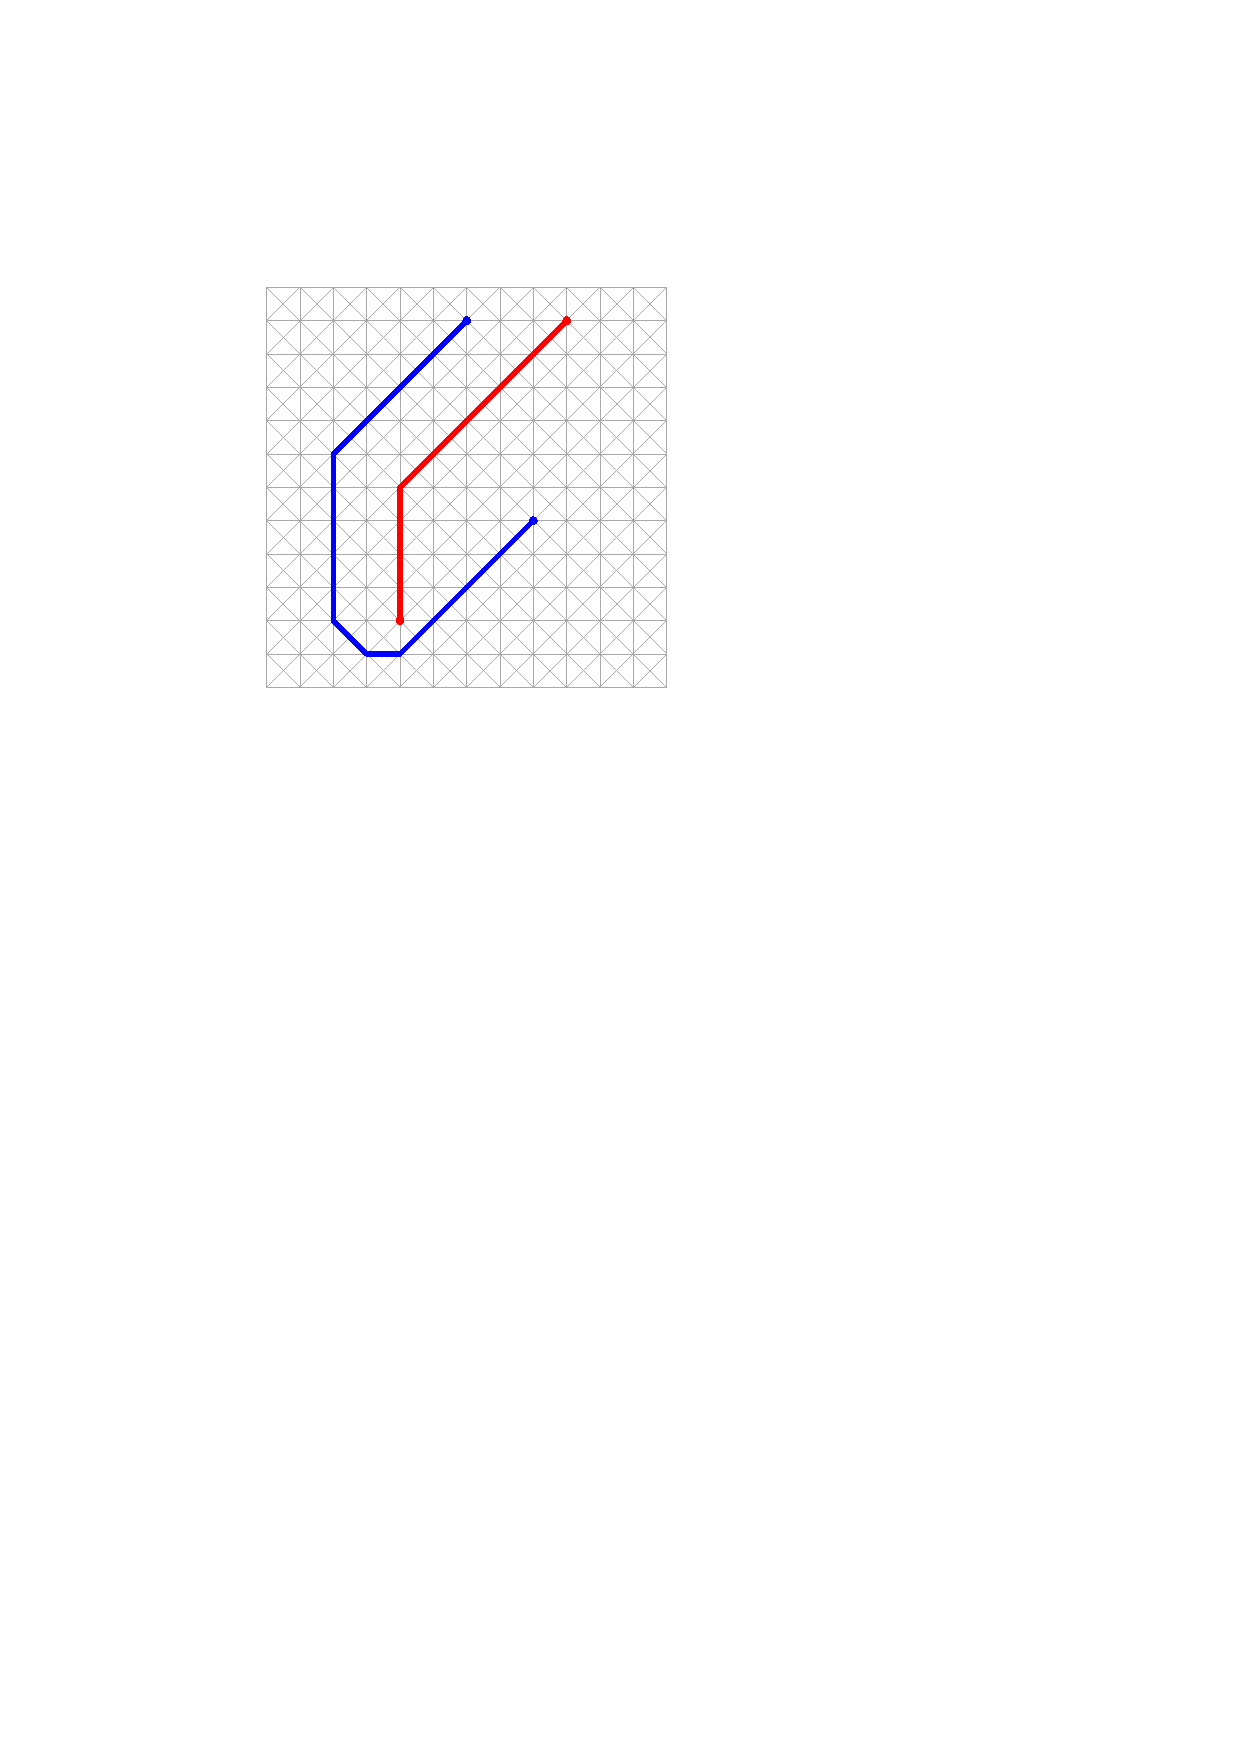
\includegraphics[width=0.474\textwidth]{figures/grid.pdf}}}$
	\caption{Left: A shortest path between $t$ and $u$ on a grid graph with uniform edge cost. Path turns are not minimized. Right: Two shortest path between $(t, u)$, and $(v, w)$ on our octilinear grid graph with uniform grid edge cost $1$ and additional path turn penalties $p_{135} = 1$, $p_{90} = 3$ and $p_{45} = 9$. Path $(t, u)$ acts as an obstacle for $(v, w)$.}
	\label{FIG:grids}
\end{figure}
\begin{figure*}[t]
  \centering
	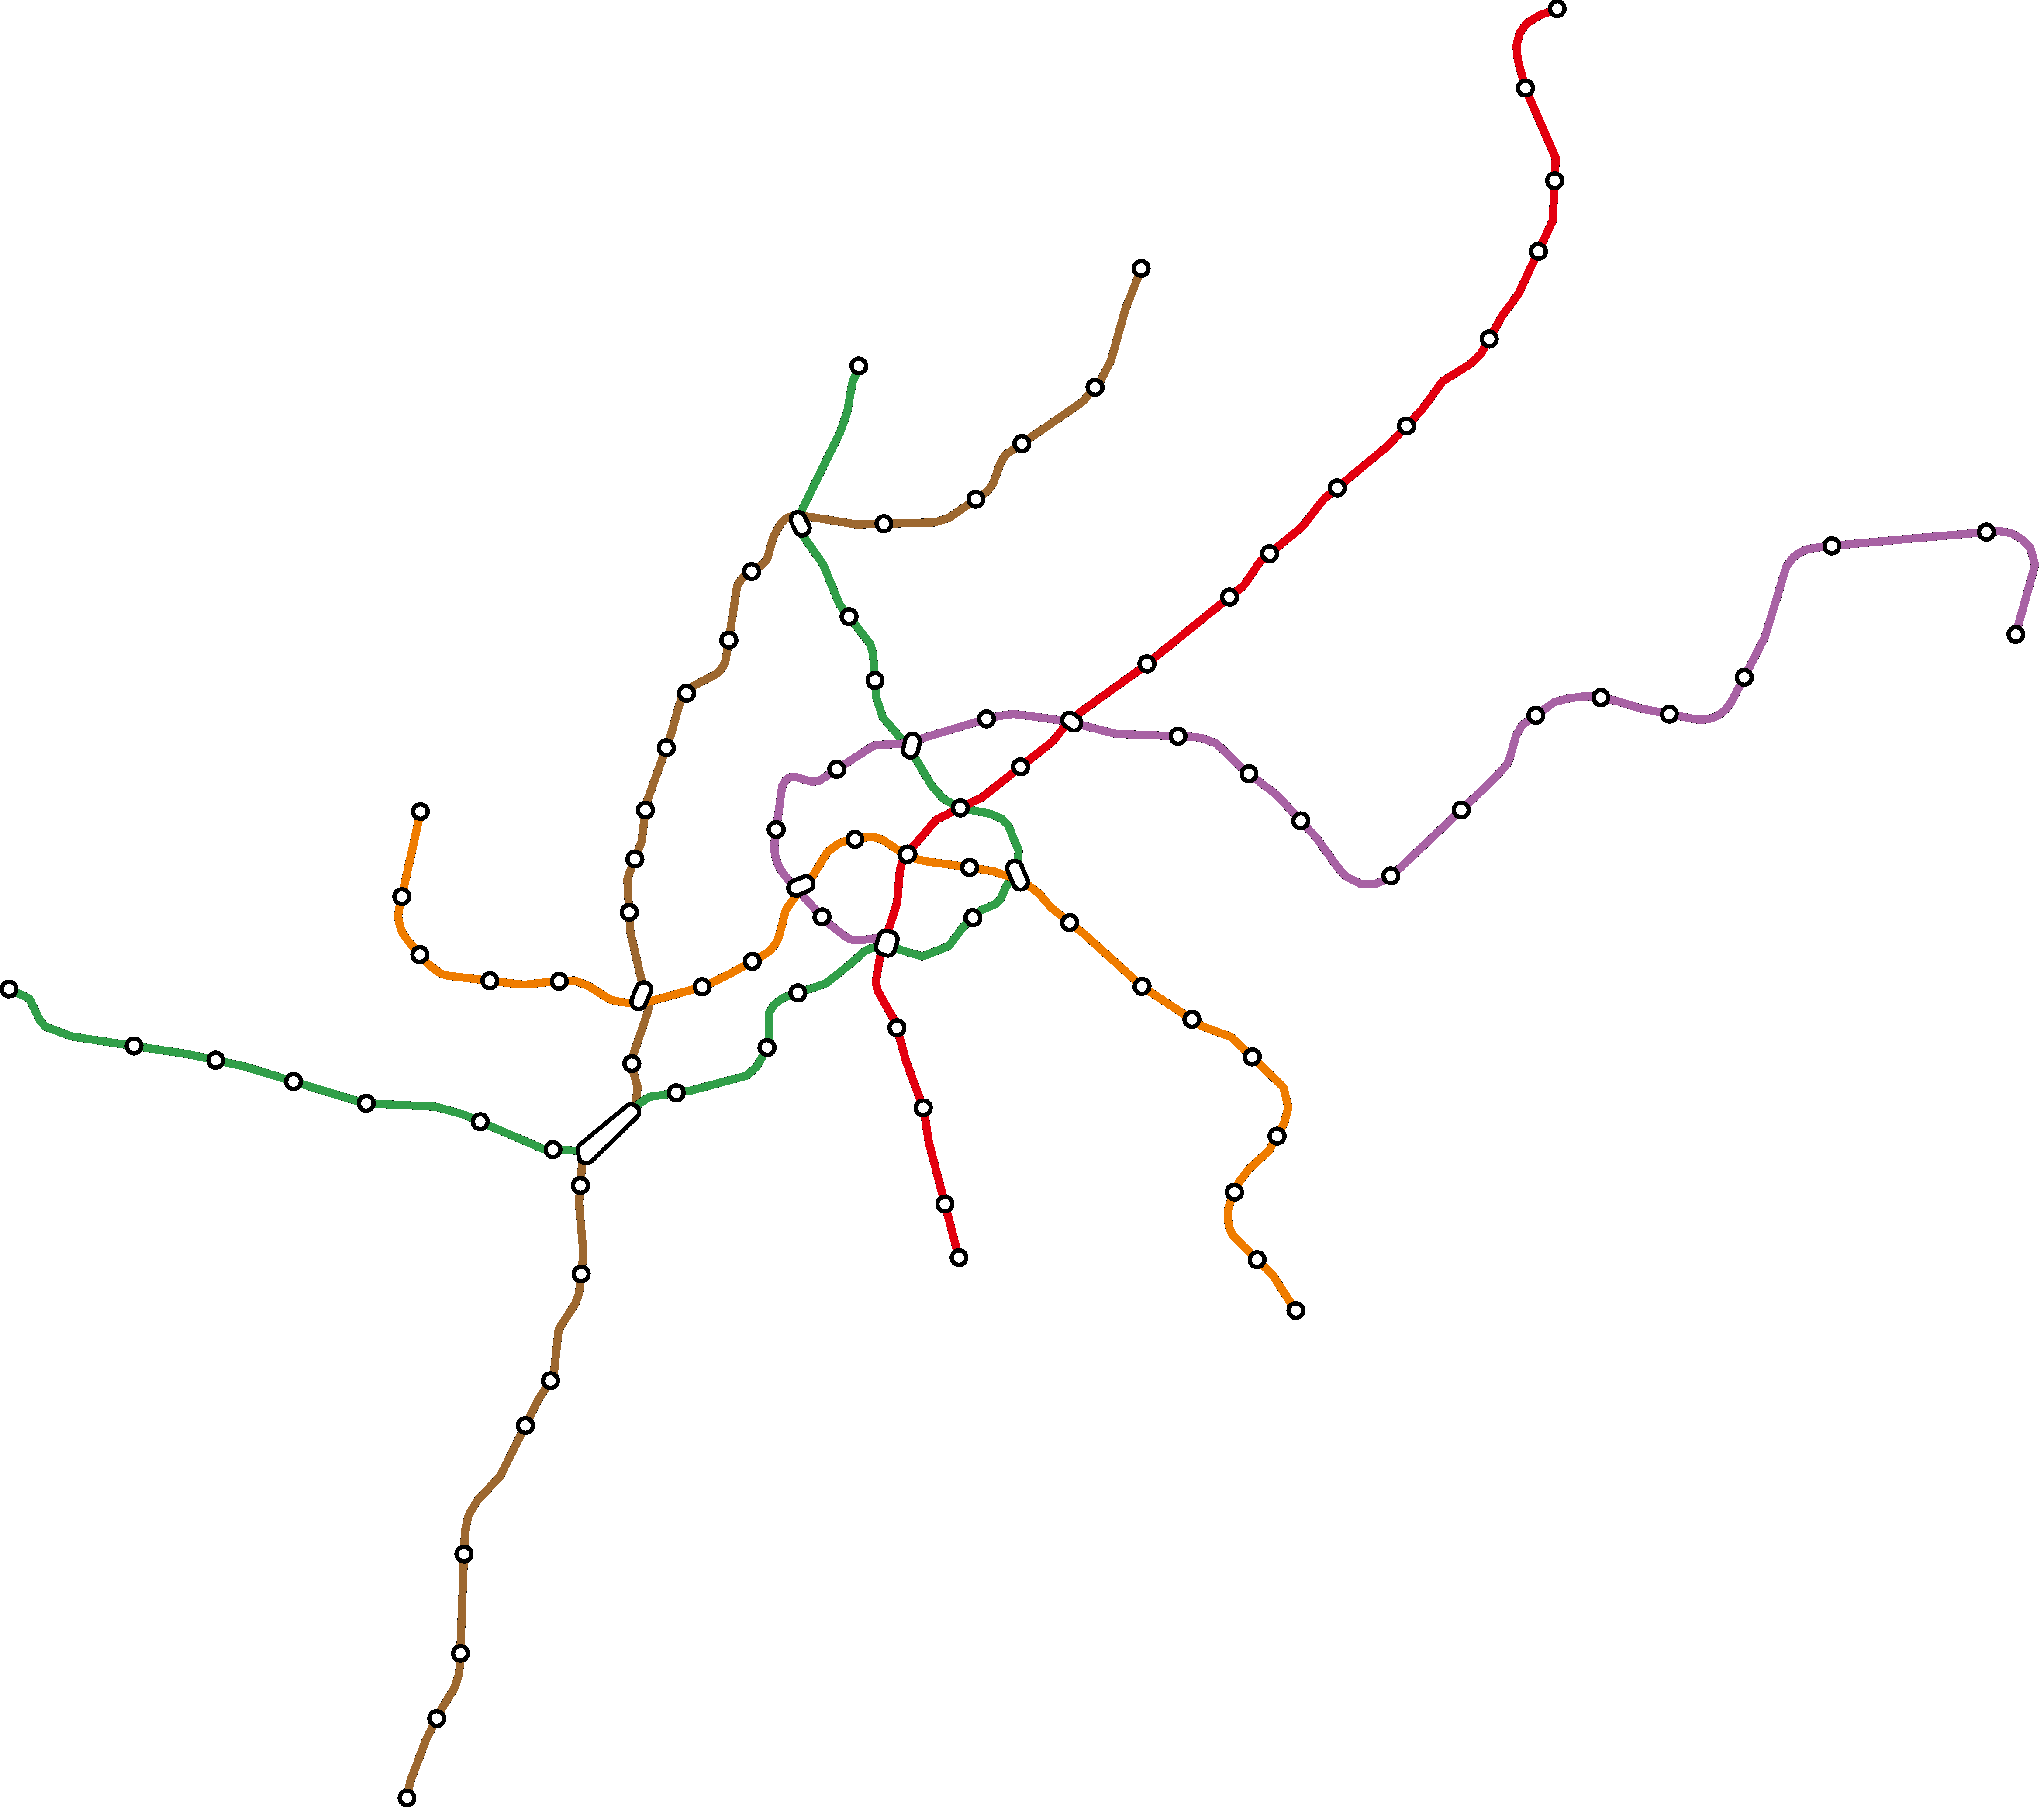
\includegraphics[width=0.474\textwidth]{figures/octi_input.pdf}
	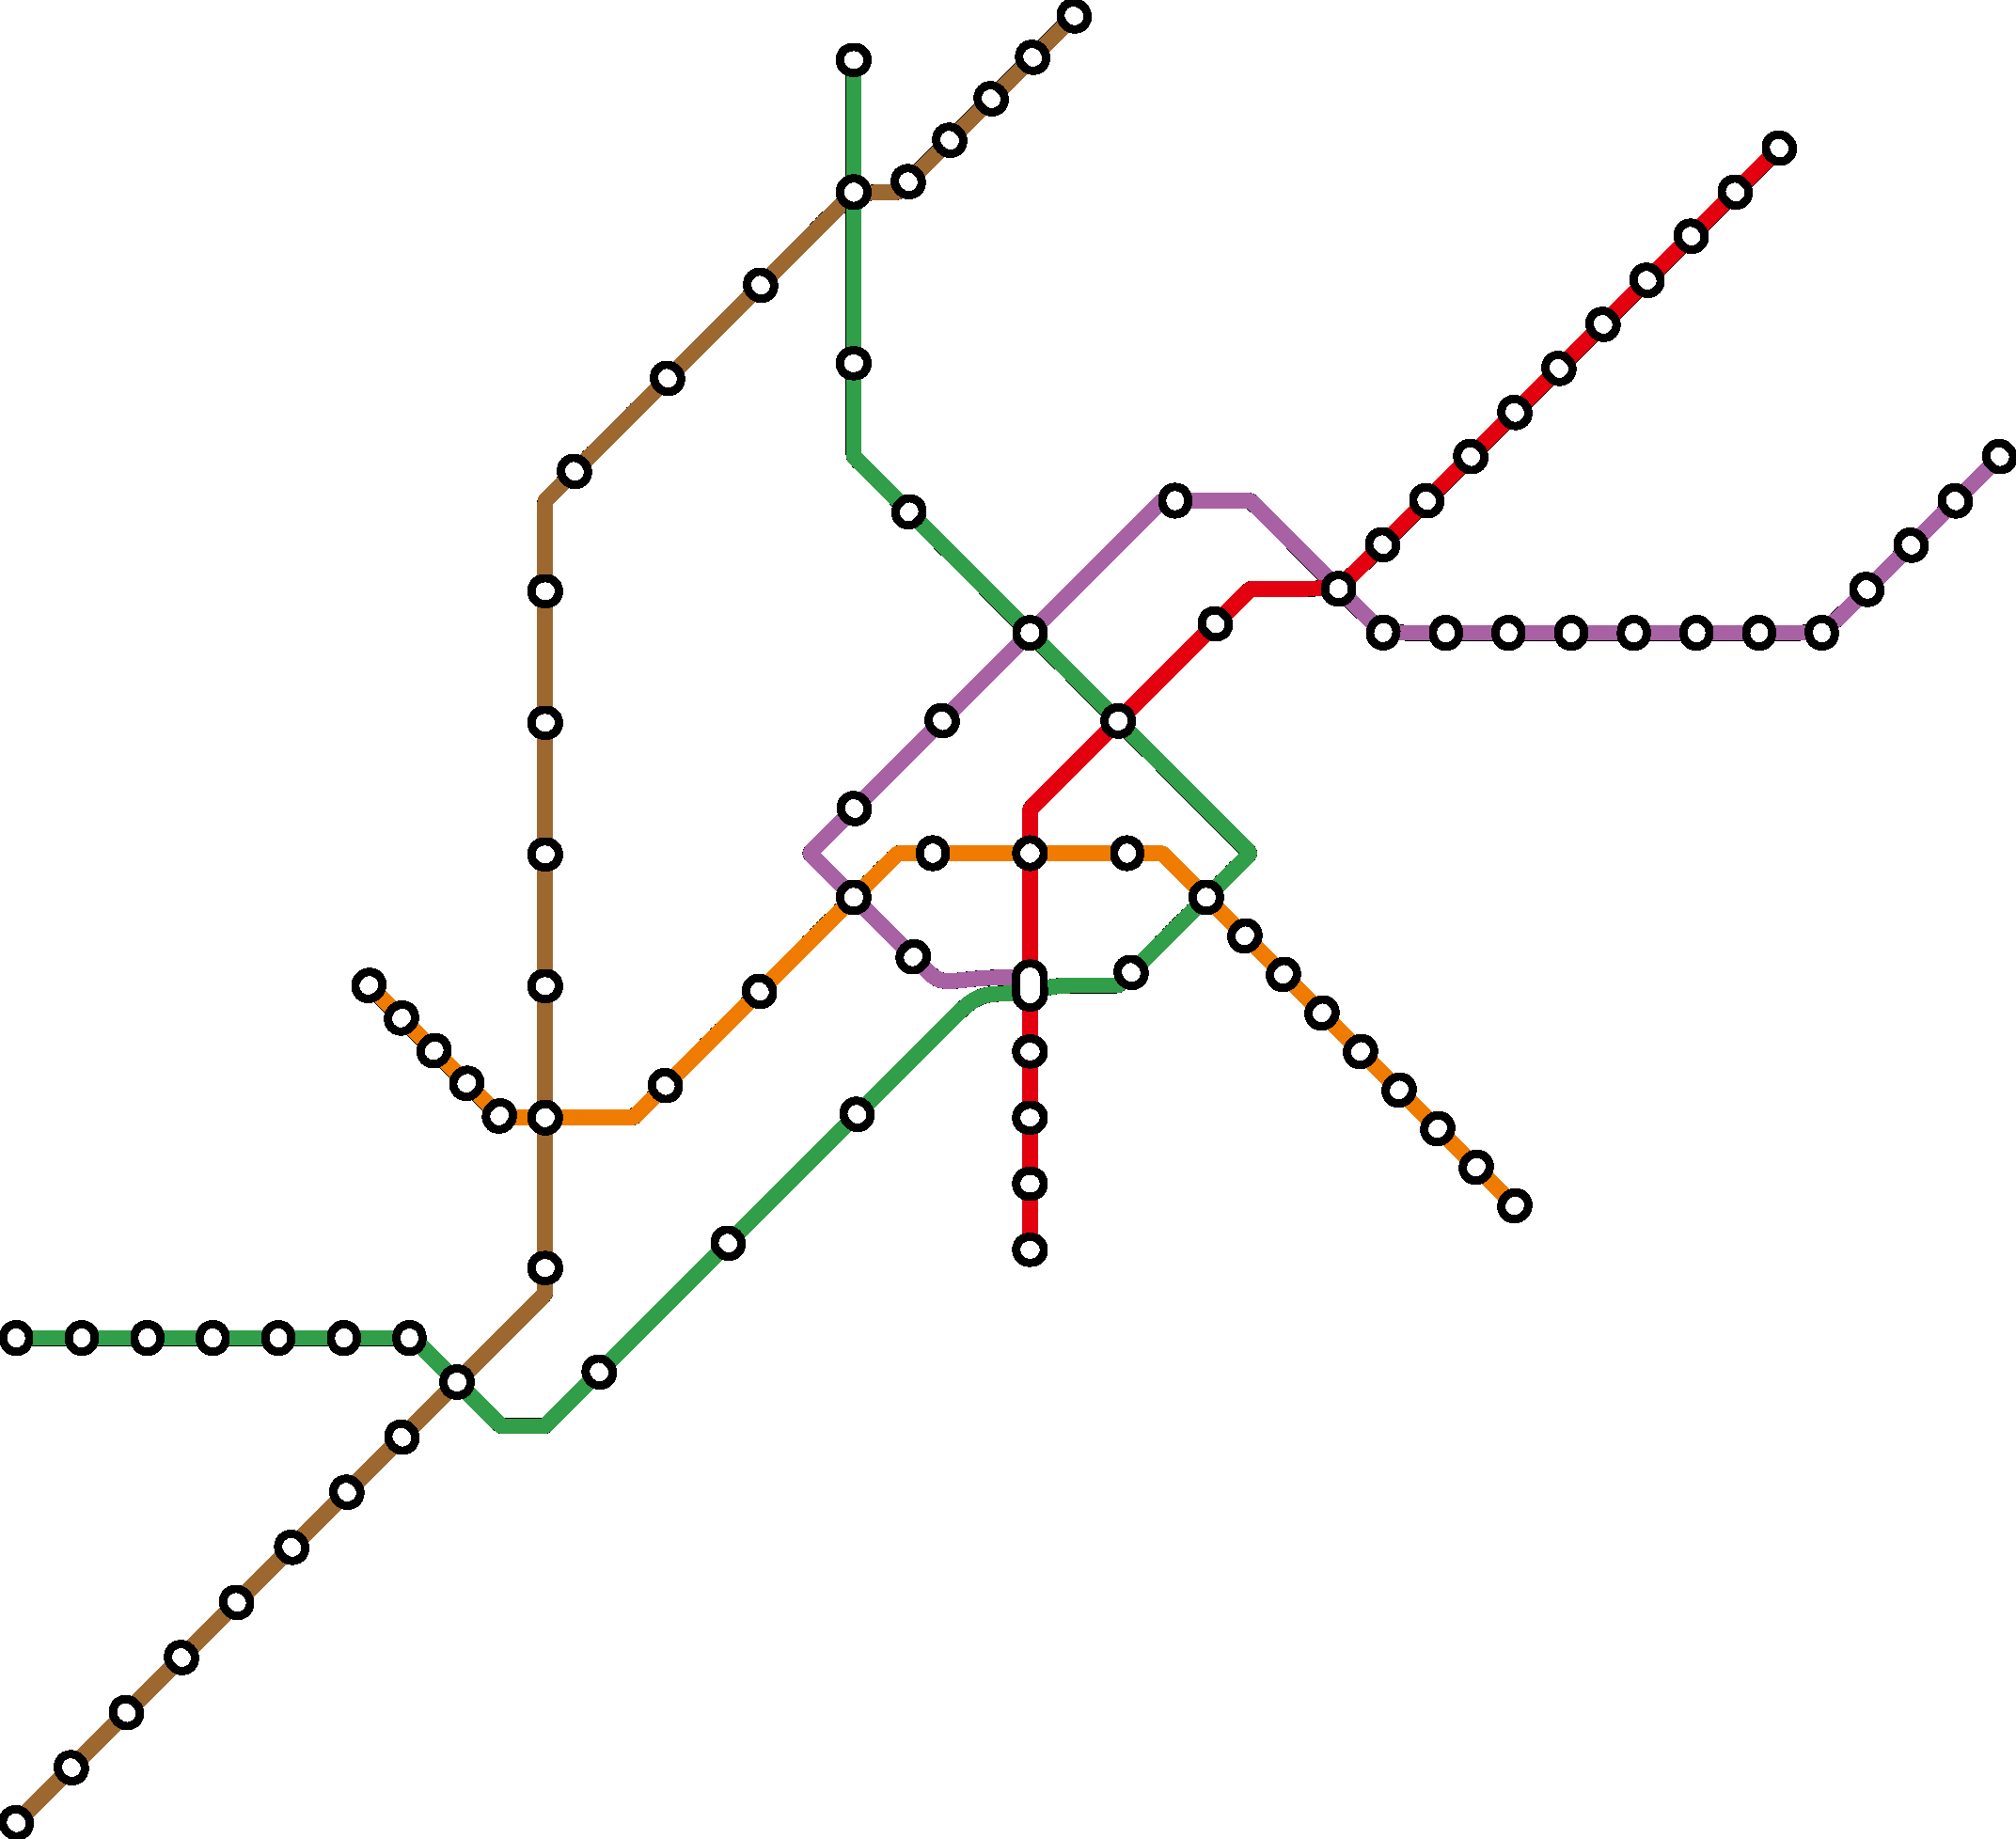
\includegraphics[width=0.474\textwidth]{figures/octi.pdf}
	\caption{The subway network of Vienna, rendered with our approach from raw timetable (GTFS) data (including stop positions).}
	\label{FIG:examplewien}
\end{figure*}

We use an auxiliary undirected graph $\Omega = \{V_\omega, E_\omega\}$ on which every possible path $p = (v_0, v_1, ..., v_n), v_i \in V_\Omega$ with $v_0 \neq v_n$ and $|p| > 1$ represents an octilinear curve with cost $c(p) = (|p| - 1) \cdot c_h$, where $c_h$ is the cost of using a single edge (note that a path consisting of $n$ nodes always uses $n - 1$ edges, so for a uniform edge cost $c_h = 1$, $c(p)$ is exactly the number of used edges).
The graph in Fig.~\ref{FIG:gridgraph},~left trivially satisfies this: we define a $x\times y$ grid and add nodes $v_{x,y}$ to $V_\omega$ for every grid point.
Each node $v_{x,y}$ is connected with its 8 direct neighbors (except at the grid boundaries) $n^0(v_{x,y}) ... N^7(v_{x, y})$, where $N^0(v_{x, y})$ is the ``north'' neighbor of $v_{n, m}$,  $N^1(v_{x, y})$ the ``north-east'' neighbor and so on, in clockwise fashion.

To later be able to optimize soft constraint (1), we additionally want the total cost for a path in $\Omega$ to reflect the number and accuteness of turns.
The penalty for a turn should be weighted by its degree - either $135^{\circ}$, $90^{\circ}$ or $45^{\circ}$.
We call these penalties $c_{135}$, $c_{90}$ and $c_{45}$.
A straight pass through a node should go unpunished, that is, $c_{180} = 0$.
Since we aim for a ``smooth'' path through $G$ and want to favor obtuse angles, we require $c_{180} \leq c_{135} \leq c_{90} \leq c_{45}$.

Formally, we now search for the path $p = (v_0, v_1, ..., v_i, ..., v_n)$ with minimum cost
\begin{align}
	c(p) = (|p| - 1) \cdot c_h + \sum_{i=1}^{n - 1} t(v_{i-1}, v_{i+1}),
\end{align}
where $t(v_{i-1}, v_{i+1})$ is the angular turn cost between edges $\{v_{i-1}, v_{i}\}$ and $\{v_{i}, v_{i=1}\}$, that is, either 0, $c_{135}$, $c_{90}$ or $c_{45}$.


We model this by adding 8 auxiliary port nodes $v_{x,y}^{0} ... v_{x,y}^{7}$ to every grid node $v_{x,y} \in V_\omega$.
Each port again corresponds to an outgoing angle in clockwise fashion and is connected to $v_{x, y}$ via sink edges $e_{x,y}^0 ... e_{x,y}^7$.
These sink edges allow us to leave from and arrive at an original node $v_{x, y}$.
For paths passing through $v_{x, y}$, we connect each port $v_{x, y}^i$ with its 7 - i suceeding (in clockwise fashion) sibling ports with turn edges $e_{x, y}^{i@45}$, $e_{x, y}^{i@90}$, and so forth.
For ease of notation, we allow a turn edge to be identified by both its port nodes, for example, $e_{x, y}^{0@45} = e_{x, y}^{1@45}$.

\begin{figure}[b]
  \centering
	$\vcenter{\hbox{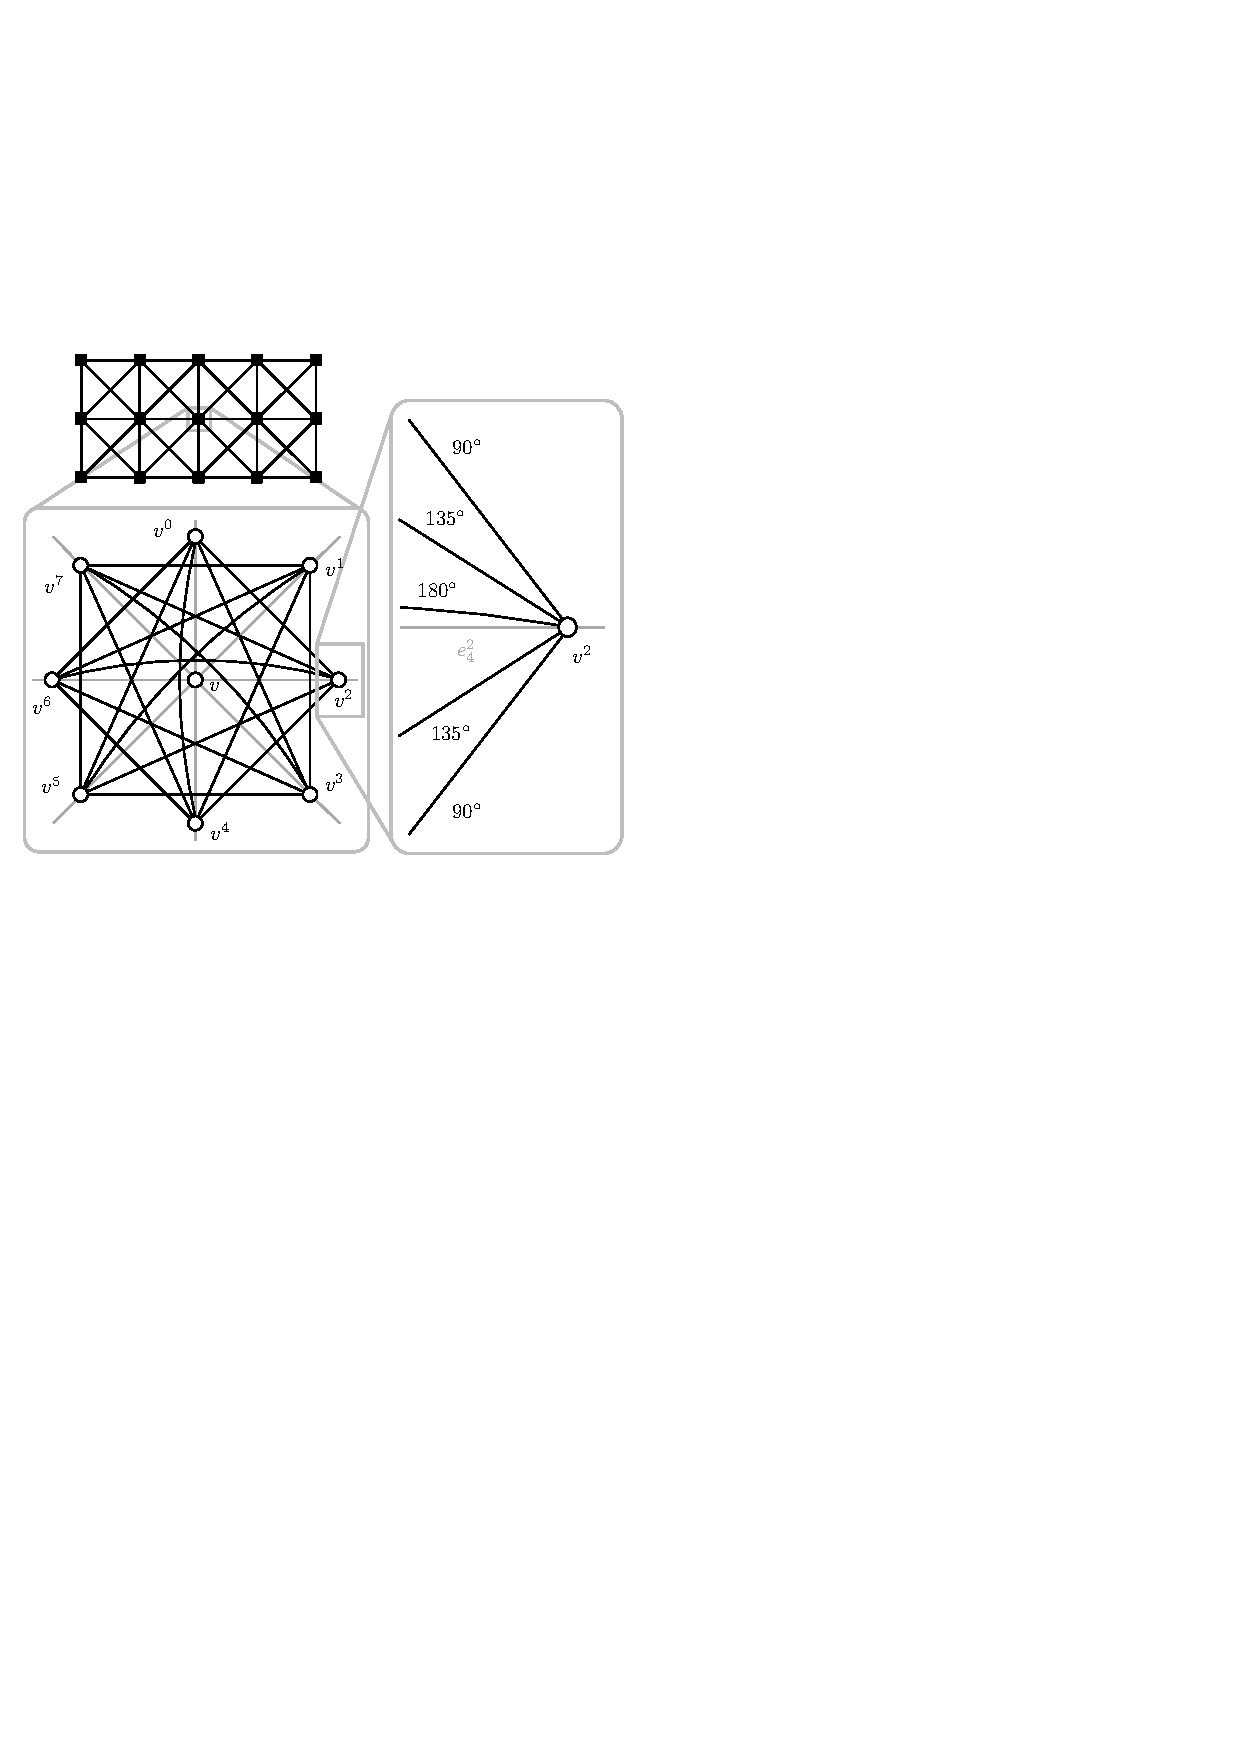
\includegraphics[width=0.45\textwidth]{figures/node.pdf}}}$
	\caption{A $3\times3$ grid graph. Each node $v_i$ has 8 ports $v_i^0 ... v_i^7$ which are connected to $v_i$ by a direct edge. Each port is additionally connected to its $180^{\circ}$, $135^{\circ}$ and $35^{\circ}$ neighbor ports.}
	\label{FIG:gridgraph}
\end{figure}

To be able to distinguish the different node and edge types, we define the set of original grid nodes as $V^g_\omega \ni v_{x, y}$, the set of port nodes as $V^p_\omega \ni v_{x,y}^i$, the set of turn edges as $E^t_\omega \ni e_{x, y}^{i@\theta}$, the set of sink edges as $E^s_\omega \ni e_{x,y}^i$ and the set of original grid edges as $E^g_\omega \ni e_{x,y}$.
Note that $V_\omega = V^g_\omega \cup V^p_\omega$ and $E_\omega = E^t_\omega \cup E^s_\omega \cup E^g_\omega$.

Additionally, for each $v \in V_\omega$, we define $v^* \in ^g_\omega$ as the original grid node belonging to $v$ (note that this may be $v$ itself).

As we want to prevent the use of sink edges in pass-through nodes, we set a uniform sink edge cost $c_s$ high enough so that a sink edge is always more expensive than a turn edge. 
In a shortest path, the only sink edges are then a leaving sink edge adjacent to $s$ and an arriving sink edge adjacent to $t$.

As both a $45^{\circ}$ port edge and a $90^{\circ}$ port edge may be substituted by cheaper edges, special care has to be applied to the modelling of the actual edge costs.
For example, a $45^{\circ}$ turn can be simulated by first passing $v_{x, y}$ on a $180^{\circ}$ port edge, and then again on a $135^{\circ}$ port edge (Fig.~\ref{FIG:paths}, 3).
As $p_{180} < p_{135} < p_{45}$, this path may be cheaper than $p_{45}$, undermining our penalty system. 
Similarily, a $90^{\circ}$ degree turn can be simulated by two cheaper $135^{\circ}$ port edges (Fig.~\ref{FIG:paths}, 4).

To prevent the shortcuts described above, we first introduce a constant $a \geq 0$ and set new port edge costs $c'_{180}, ..., c'_{45}$ as follows:
%
\begin{align}
	c'_{180} &= a + c_{180} = a \\
	c'_{135} &= a + c_{135} \\
	c'_{90} &= a + c_{90} \\
	c'_{45} &= a + c_{45}.
\end{align}
%
We choose $a$ in a way such that the following inequalities are fullfilled:
%
\begin{align}
	2a + 2c_{135} &\geq a + c_{90} \label{CONSTRS:sim90}\\
	2a + c_{135} + c_{90} &\geq a + c{45}\label{CONSTRS:sim45}.
\end{align}
Ineq.~(\ref{CONSTRS:sim90}) ensures that simulating a $90^{\circ}$ pass with two $135^{\circ}$ passes is never cheaper than $c_{90}$.
Ineq.~(\ref{CONSTRS:sim45}) ensures that simulating a $45^{\circ}$ pass with a $135^{\circ}$ pass and a $180^{\circ}$ pass is never cheaper than $c_{45}$.

The inequalities are fullfilled for $a = c_{45} - c_{135}$.

The shortest path $p'$ from an original grid node $s = v_0 \in V^s_\omega$ to another original grid node $t=v_n \in V^s_\omega$ on our octilinear grid graph now consists of \emph{two} nodes for each original grid node: for the start and end node, the original node and a single port node appear in the path.
For pass-through nodes, a port node for arriving at and a port node for leaving the original grid node appears (w.l.o.g., we ignore the case where a turn edge is replaced by two turn costs with similar cost, as this does neither affect the final path on the grid graph, nor the cost of that path).

This shortest path $p' = (v_0, v_1, ..., v_n')$ thus always describes a path $p = (v^*_0, v^*_2, v^*_4, ..., v^*_{n'/2})$ on the original grid graph with $|p| = n = |p'| / 2 = n' / 2$ and has the cost
%
\begin{align}
	c'(p') = 2 c_s + \left(n - 1\right) \cdot c_h + \sum_{i=1}^{n - 1} a + t\left(v^*_{2i - 2}, v^*_{2i+2}\right)\label{EQ:cost}.
\end{align}
%
To get rid of the constant offset $a$, we set $c_{135} = 1$, $c_{90} = 1.5$ and $c_{45} = 2$, which means $a = 1$.
If we then set the cost of a single grid edge $c_h = 1 = a$ and set the actual grid edge costs to $c'_h = c_h - a = 0$, we can rewrite Eq.~\ref{EQ:cost} as  
%
\begin{align}
	c'(p') &= 2 c_s +  \left(n - 1\right) \cdot c'_h + \sum_{i=1}^{n - 1} c_h + t\left(v^*_{2i - 2}, v^*_{2i+2}\right) \\
	     &= 2 c_s + \left(n - 2\right) \cdot c_h + \sum_{i=1}^{n - 1} t \left(v^*_{2i - 2}, v^*_{2i+2}\right) \\
	     &= 2 c_s + c(p) - c_h = c(p) + 2 c_s - 1.
\end{align}
%
As $p'$ minimizes $c(p) + 2 c_s - 1$, it also minimizes $c(p)$.

\begin{figure*}[h]
  \centering
	$\vcenter{\hbox{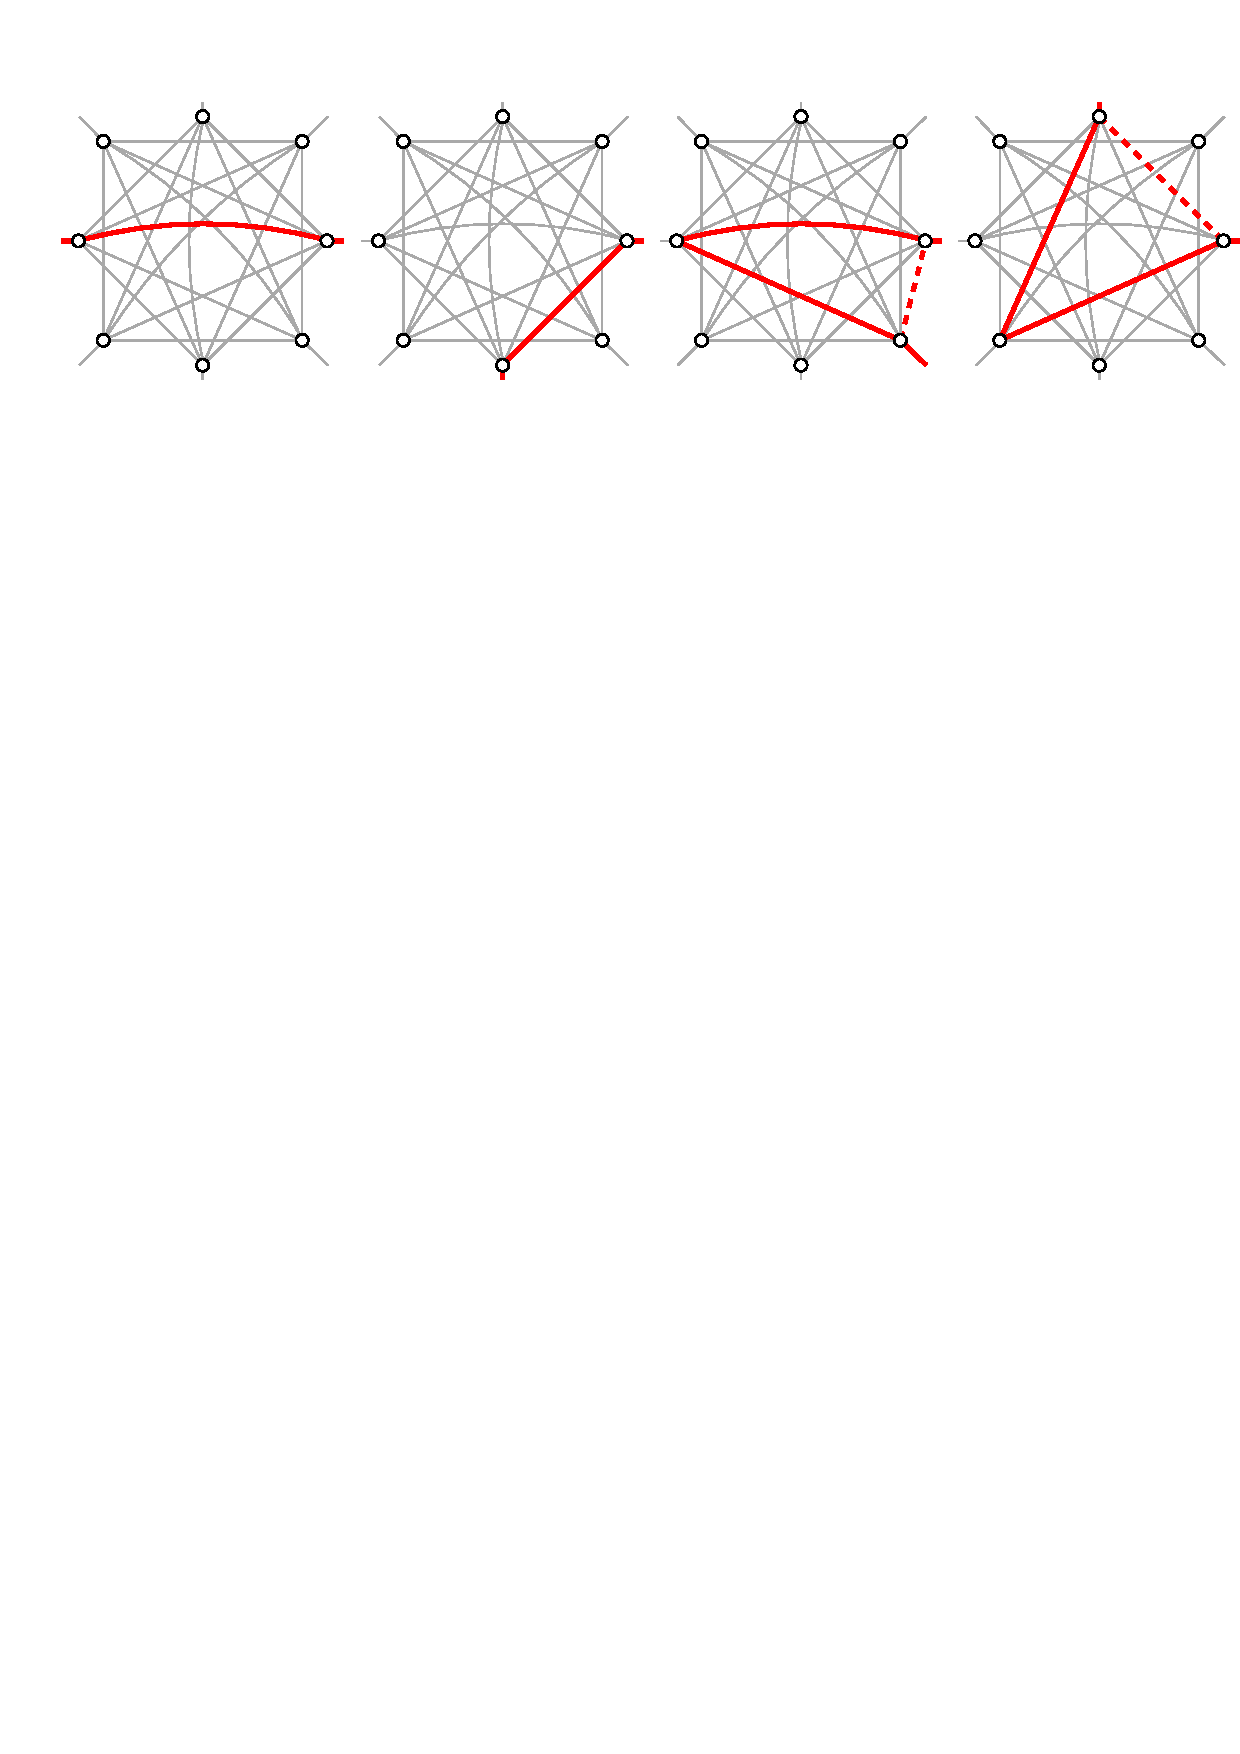
\includegraphics[width=0.9\textwidth]{figures/paths.pdf}}}$
	\caption{1. A $180^{\circ}$ pass through a node $v$. 2. A $90^{\circ}$ pass through $v$. 3. A $45^{\circ}$ pass through $v$ simulated by a $180^{\circ}$ and $135^{\circ}$ pass. 4. A $90^{\circ}$ pass through $v$ simulated by two $135^{\circ}$ passes. }
	\label{FIG:paths}
\end{figure*}

\section{Optimal Solution via ILP}

Using the octilinear grid graph $\Omega$ from the previous section, we can now define the problem of finding the optimal metro-map drawing on the grid defined by $\Omega$ like this: find the grid position for each input station and the shortest paths between adjacent input station nodes which minimizes the sum of (1) all shortest path costs, (2) the distance between the grid position of a station and its original position, and (3) the line bend penalties at stations (which are not covered by the path costs on $\Omega$).
The input embedding should be preserved, which means that the circular ordering of the input edges at nodes should be preserved, and the shortest paths should be non intersecting.

We first describe how to solve this problem exactly using an Integer Linear Program (ILP).

\subsection{Station Placement}

\subsection{Edge Continuity}

\subsection{Preservement of Embedding}

\subsection{Avoiding Line Bends}

\subsection{Complexity}

\section{Approximative Solution}

\subsection{Station Placement}

\subsection{Edge Continuity}

\subsection{Preservement of Embedding}

\subsection{Avoiding Line Bends}

\subsection{Optimization via Local Search}

\subsection{Complexity}

\section{Evaluation}

\subsection{Penalty Experiments}

\section{Conclusions}


\balancecolumns
\end{document}
